\section{Bike model of vehicle}
The nonlinear dynamics that we adopt as being the "ground truth" for the ego vehicle's movement are given by a 7D kinematic bicycle model.
The model considers that the two front wheels and two rear wheels of the vehicle move in unison, with steering provided by the front wheels only. 
Furthermore, each abstracted wheel is located along the center of the vehicles body and does not slip. 

Figure \ref{fig:bike} shows the state variables and parameters involved in the model.

\begin{figure}[t]
	\centering
	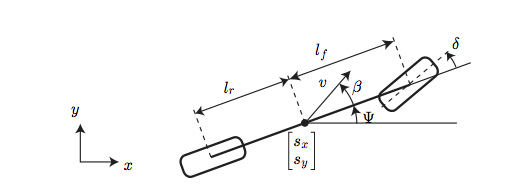
\includegraphics[scale=0.5]{figures/bicycle}
	\caption{Bicycle Model of the Ego Vehicle \cite{Althoff2014}}
	\label{fig:bike}
\end{figure}

\begin{table}[h]
	\label{table:vehiclep}
	\begin{tabular}{|c|c|c|c|c|c|}
		\hline
		\multicolumn{6}{|c|}{Vehicle Parameters} \\ \hline
		\textit{$m$} & \textit{$I_z$} & \textit{$C_f$} & \textit{$C_r$} & \textit{$l_f$} & \textit{$l_r$} \\ \hline
		2273 kg & 4423 kg*m$^2$ & 10.8e4 N/rad & 10.8e4 N/rad & 1.292 m & 1.515 m \\ \hline
	\end{tabular}
	\caption{Parameters of Example Ego Vehicle}
\end{table}

The parameters \(C_f,C_r\) and \(l_f, l_r\) describe respectively the cornering stiffness and distances from the center of gravity to the axles respectively. The moment of inertia, \(I_z\) and the vehicle mass, \(m\) are experimentally determined constants \cite{Snider2009}. 
The parameters of the model can be experimentally determined and validated.
Their values for the Cadillac SRX model, as reported by \cite{Althoff2014}, are shown in Table \ref{table:vehiclep}.

The variable \(\beta\) is the slip angle at the center of mass, \(\psi\) is the heading angle, \(\dot{\psi}\) is the yaw rate, \(v\) is the velocity, \(s_x\) and \(s_y\) are the x and y positions, and \(\delta\) is the angle of the front wheel. 
In the formulation of \cite{Althoff2014}, the inputs to the system are \(a_x\), the longitudinal acceleration, and \(v_w\) the rotational speed of the steering angle. The \(y\) terms represent disturbances to the system. 
For example \(y_{\beta}\) and \(y_{\dot{\psi}}\) represent disturbances to the slip angle at the center of mass and the yaw rate. The state equations for the system are:
\begin{gather*}
\label{eqn:beta}
\dot{\beta}=\left(\frac{C_rl_r-C_fl_f}{mv^2} \right)\dot{\psi}+\left(\frac{C_f}{mv} \right)\delta-\left(\frac{C_f+C_r}{mv} \right)\beta+y_{\beta}
\\
\label{eqn:psi}
\ddot{\psi}=\left(\frac{C_rl_r-C_fl_f}{I_z} \right)\beta-\left(\frac{C_fl_f^2-C_rl_r^2}{I_z} \right)\left(\frac{\dot{\psi}}{v} \right)+\left(\frac{C_fl_f}{I_z} \right)\delta+y_{\dot{\psi}}
\\
\label{eqn:v}
\dot{v}=a_x+y_v
\\
\label{eqn:sx}
\dot{s_x}=v\cos{(\beta+\psi)}+y_{s_x}
\\
\label{eqn:sy}
\dot{s_y}=v\sin{(\beta+\psi)}+y_{s_y}
\\
\label{eqn:delta}
\dot{\delta}=v_w+y_d
\end{gather*}


\subsection{Tracking Controller}
The scenario model considers a simple path tracking controller which was successfully implemented and used on the CMU DARPA Grand Challenge vehicle. Path tracking controllers guide a vehicle along a geometrically defined trajectory by apply steering and longitudinal acceleration inputs. A successful path tracking algorithm maintains vehicle stability and attempts to minimize the error between the desired trajectory and actual trajectory. The parameters computed for this controller when implemented and validated on a Cadillac SRX \cite{Althoff2014}.

Thus, the feedback to the system are the lateral and longitudinal tracking errors. We derive the following results as in  \cite{Snider2009}:
\begin{gather*}
\epsilon_x=cos{(\Psi_d)}(s_{x,d}-s_x) +sin{(\Psi_d)}(s_{y,d}-s_y)
\\
\epsilon_y=-sin{(\Psi_d)}(s_{x,q}-s_x)+cos{(\Psi_d)}(s_{y,d}-s_y)
\end{gather*}
Through the lateral tracking error, and desired trajectory we can then compute the desired rate of change of the angle of the front wheel with respect to time. This enables the computation of rate of change of the rotational speed of the steering angle. We note that the relevant parameters are again defined using the validated model in \cite{Althoff2014}.
\begin{gather*}
\delta_d=k_1 \epsilon_y+k_2(\Psi_d-\Psi)+ k_3(\dot{\Psi_d}-\dot{\Psi})
\\
v_w=k_4(\delta_d-\delta)
\end{gather*}
The longitudinal acceleration is simply defined by the tracking error between the actual velocity and the desired velocity.
\begin{gather*}
a_x=k_5\epsilon_x+k_6(v_d-v)
\end{gather*}
Combining the equations as in \cite{Althoff2014} the control inputs for longitudinal acceleration (pressing the accelerator) and steering angle velocity (turning the steering wheel) can be computed as $v_w$ and $a_x$ respectively. 
\begin{gather*}
v_w=k_1(cos{(\Psi_d)}(s_{y,d}-s_y-w_y)-sin{(\Psi_d)}(s_{x,d}-s_x-w_x))+k_2(\Psi_d-\Psi-w_{\Psi})\\ +k_3(\dot{\Psi_d}-\dot{\Psi}-w_{\psi})-k_4(\delta-w_{\delta})
\\
a_x=k_5(cos{(\Psi_d)}(s_{x,d}-s_x-w_x)+sin{(\Psi_d)}(s_{y,d}-s_y-w_y))+k_6(v_d-v-w_v)
\end{gather*}

\subsection{Trajectories}
To use the tracking controller in the lane change scenario, we must specify a lane change trajectory for the controller to track.
In our simple example, we use a simple hyperbola $s_{x,d} = s_{y,d}^3$ with inflection point at the current position of the car.
By substituting this into the equations above we obtain $\Psi_d$, and the closed-loop dynamics of the system. 
Other trajectories can be used and the analysis that follows is unchanged.
%In order to define a valid trajectory and controller for a lane change maneuver several constants beyond the controller parameters must be specified.
%We state that $w$ is the width of the road in meters and $v_d$ is the desired velocity of the vehicle in $m/s$. 
%We also define variable $t$ to represent time is units of seconds. 
%We then define the quantity $v_{mag}$ which is the magnitude of the vehicle's velocity vector measured in $m/s$.
%For convenience, we compute the magnitude of the velocity vector at time $t$.
%\begin{gather*}
%v_{mag}=\sqrt{9(t-.5w)^4 +1}
%\end{gather*}
%
%The individual quantities of $\dot{s_{x_d}}$ and $\dot{s_{y_d}}$ are as follows:
%\begin{gather*}
%\dot{s_{x_d}}=3v_d(t-.5w)^2/v_{mag}\\
%\dot{s_{y_d}}=v_d/v_{mag}\\
%\end{gather*}
%
%Finally the first and second derivative of the steering angle are:
%\begin{gather*}
%\dot{\Psi_d}=(48w-96t)/(81*(w-2t)^8)\\
%\ddot{\Psi_d}=96(-16+27(-2t+w)^4)/(16+9(-2t+w)^4)^2
%\end{gather*}
